%==============================================================================
%  MATH 231 -- Linear Algebra I (Fall 2026)
%  LECTURE 0 -- FOUNDATIONS REVIEW (self-study, before the course begins)
%
%  Audience: intro linear algebra students who have completed MATH 141
%  (Calculus I, with differentiation).  This lecture reviews the prerequisite
%  "language" the course assumes on Day 1: sets and notation, summation/product
%  notation, exponents/logs, polynomials, and the geometry of distance and the
%  circle.  Every idea is followed by a worked example, and short "Looking
%  ahead" notes connect the review to specific units of the course.
%
%  Compile with pdflatex (standard TeX Live packages only).
%==============================================================================
\documentclass[11pt]{article}

\usepackage[margin=1in]{geometry}
\usepackage{amsmath,amssymb,amsthm}
\usepackage[dvipsnames]{xcolor}
\usepackage{enumitem}
\usepackage{booktabs}
\usepackage{array}
\usepackage{colortbl}
\usepackage{tikz}
\usetikzlibrary{arrows.meta}
\usepackage[hidelinks]{hyperref}
\usepackage{titlesec}

%------------------------------------------------------------------ style ----
\titleformat{\section}{\Large\bfseries\sffamily\color{RoyalBlue}}{\thesection.}{0.6em}{}
\titleformat{\subsection}{\large\bfseries\sffamily}{\thesubsection}{0.6em}{}

\hypersetup{colorlinks=true,linkcolor=RoyalBlue,urlcolor=BrickRed}

% environments -----------------------------------------------------------------
\theoremstyle{definition}
\newtheorem{example}{Example}[section]

% a boxed "key facts" panel
\newcommand{\keybox}[2]{%
  \par\smallskip\noindent
  \begin{tabular}{@{}p{0.985\linewidth}@{}}
  \arrayrulecolor{RoyalBlue}\toprule
  {\sffamily\bfseries\color{RoyalBlue}#1}\\[2pt]#2\\
  \bottomrule
  \end{tabular}\par\smallskip}

% forward-reference note tying review to the course
\newcommand{\lookahead}[1]{%
  \par\smallskip\noindent
  {\sffamily\bfseries\color{BrickRed}Looking ahead.~}\textit{#1}\par\smallskip}

\newcommand{\R}{\mathbb{R}}
\newcommand{\C}{\mathbb{C}}
\newcommand{\Z}{\mathbb{Z}}
\newcommand{\N}{\mathbb{N}}
\newcommand{\Q}{\mathbb{Q}}
\newcommand{\ds}{\displaystyle}

\title{\vspace{-1.2cm}\textbf{\sffamily MATH 231 -- Linear Algebra I}\\[4pt]
       {\large\sffamily Foundations Review}\\[2pt]
       {\normalsize\sffamily A self-study primer to read \emph{before} the course begins}}
\author{}
\date{\normalsize\sffamily Fall 2026}

\begin{document}
\maketitle
\vspace{-1.0cm}

%==============================================================================
\section*{Before you start}
%==============================================================================
This is a \textbf{primer}: it contains no new linear algebra. Everything
here is material you have seen before, gathered in one place so that on Day~1 we
can speak a common language. Your only formal prerequisite is \textbf{MATH~141}
(Calculus~I). If a page feels like review, skim it; if a page feels new, slow
down and work the examples with a pencil --- that is the whole point of a primer.

\keybox{How to use this document}{%
Read actively. For every \emph{Example}, cover the solution and try it first.
The \textcolor{BrickRed}{\textbf{\textsf{Looking ahead}}} notes tell you
\emph{why} a piece of review matters --- each points to the unit of MATH~231
where the idea returns with full force. A short self-check with answers is at the
end.}

\tableofcontents
\bigskip

%==============================================================================
\section{Numbers and Sets}
%==============================================================================

\subsection{The number systems}
We build up from the counting numbers to the real line, each system fixing a
shortcoming of the previous one.
\[
\underbrace{\N}_{\text{naturals}}\subset
\underbrace{\Z}_{\text{integers}}\subset
\underbrace{\Q}_{\text{rationals}}\subset
\underbrace{\R}_{\text{reals}}\subset
\underbrace{\C}_{\text{complex}}
\]
\begin{itemize}[leftmargin=1.4em,itemsep=1pt]
  \item $\N=\{0,1,2,3,\dots\}$ (in this course we include $0$; some books start at $1$).
  \item $\Z=\{\dots,-2,-1,0,1,2,\dots\}$ --- adds subtraction.
  \item $\Q=\bigl\{\tfrac{p}{q}: p,q\in\Z,\ q\neq 0\bigr\}$ --- adds division.
  \item $\R$ --- fills the ``gaps'' (e.g.\ $\sqrt{2}$, $\pi$, $e$ are real but not rational).
  \item $\C=\{a+bi: a,b\in\R,\ i^2=-1\}$ --- adds roots of \emph{every} polynomial.
\end{itemize}
\lookahead{A vector space (Unit~1) is always built \emph{over} a number system
called its field of scalars --- almost always $\R$ or $\C$. Complex numbers get
their own treatment in Unit~3, where $i^2=-1$ becomes rotation by $90^\circ$.}

\subsection{Sets, elements, and membership}
A \textbf{set} is an unordered collection of distinct objects called its
\textbf{elements}. We write:
\[
x\in A \quad(\text{``$x$ is an element of $A$''}), \qquad
x\notin A \quad(\text{``$x$ is not an element of $A$''}).
\]
Two ways to describe a set:
\begin{itemize}[leftmargin=1.4em,itemsep=1pt]
  \item \textbf{Roster (list) form:} $A=\{2,4,6,8\}$.
  \item \textbf{Set-builder form:} $A=\{\,x : \text{condition on }x\,\}$, read
        ``the set of all $x$ \emph{such that} \dots''. The colon ``$:$'' (or
        ``$\mid$'') means \emph{such that}.
\end{itemize}

\begin{example}
Write ``the even numbers between $1$ and $9$'' in set-builder form.
\[
A=\{\,x\in\Z : 1\le x\le 9 \text{ and } x \text{ is even}\,\}=\{2,4,6,8\}.
\]
The part before the colon says \emph{what kind} of object ($x\in\Z$); the part
after says \emph{which ones} we keep.
\end{example}

\begin{example}
The unit circle is a set of points: $\;S=\{(x,y)\in\R^2 : x^2+y^2=1\}$. This is
the same object as the geometric circle of \S7 --- a \emph{set} and an
\emph{equation} describing the same thing.
\end{example}

The \textbf{empty set} $\varnothing=\{\ \}$ has no elements. The number of
elements of a finite set $A$ is its \textbf{cardinality} $|A|$; e.g.\
$|\{2,4,6,8\}|=4$.

\lookahead{Set-builder notation is how we will \emph{define} the central objects
of the course: a span, a subspace, a null space, and the feasible region of an
optimization problem are all written $\{\,x : \text{some linear condition}\,\}$.}

\subsection{Subsets and equality}
$A$ is a \textbf{subset} of $B$, written $A\subseteq B$, if every element of $A$
is also in $B$. If in addition $A\neq B$ we call it a \textbf{proper subset},
$A\subsetneq B$. Two sets are \textbf{equal} exactly when each contains the other:
\[
A=B \iff (A\subseteq B \text{ and } B\subseteq A).
\]
This ``two-way inclusion'' is the standard way to \emph{prove} two sets are equal.

\begin{example}
Let $A=\{1,2\}$ and $B=\{1,2,3\}$. Then $A\subseteq B$ (indeed $A\subsetneq B$),
but $B\not\subseteq A$ since $3\in B$ but $3\notin A$. Also $\varnothing\subseteq A$
for \emph{every} set $A$.
\end{example}

\subsection{Set operations}
Given sets $A,B$ inside some universe $U$:
\[
\begin{array}{lll}
\textbf{Union} & A\cup B=\{x: x\in A \text{ or } x\in B\} & \text{everything in either}\\[2pt]
\textbf{Intersection} & A\cap B=\{x: x\in A \text{ and } x\in B\} & \text{the overlap}\\[2pt]
\textbf{Difference} & A\setminus B=\{x: x\in A \text{ and } x\notin B\} & \text{in $A$ but not $B$}\\[2pt]
\textbf{Complement} & A^{c}=U\setminus A=\{x\in U: x\notin A\} & \text{everything outside $A$}
\end{array}
\]

\begin{center}
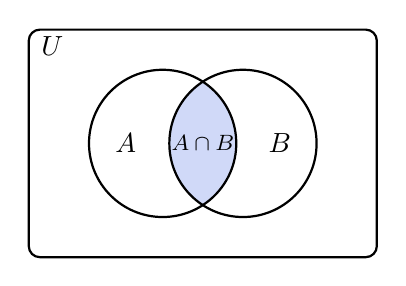
\begin{tikzpicture}[scale=0.85]
  \draw[rounded corners,thick] (-2.6,-1.7) rectangle (2.6,1.7);
  \node at (-2.25,1.45) {$U$};
  \begin{scope}
    \clip (-0.6,0) circle (1.1);
    \fill[RoyalBlue!25] (0.6,0) circle (1.1);
  \end{scope}
  \draw[thick] (-0.6,0) circle (1.1);
  \draw[thick] (0.6,0) circle (1.1);
  \node at (-1.15,0) {$A$};
  \node at (1.15,0) {$B$};
  \node[font=\footnotesize] at (0,0) {$A\cap B$};
\end{tikzpicture}
\end{center}

\begin{example}
Let $A=\{1,2,3,4\}$, $B=\{3,4,5,6\}$, universe $U=\{1,2,\dots,8\}$.
\[
A\cup B=\{1,2,3,4,5,6\},\quad A\cap B=\{3,4\},\quad
A\setminus B=\{1,2\},\quad A^c=\{5,6,7,8\}.
\]
\end{example}

The \textbf{Cartesian product} pairs elements from two sets in order:
\[
A\times B=\{(a,b): a\in A,\ b\in B\}.
\]
The plane is $\R^2=\R\times\R=\{(x,y):x,y\in\R\}$ and space is
$\R^3=\R\times\R\times\R$. Order matters: $(1,2)\neq(2,1)$.

\lookahead{$\R^n=\R\times\cdots\times\R$ ($n$ copies) is where \emph{vectors}
live (Unit~1). A vector is nothing more exotic than an ordered list of $n$ real
numbers --- an element of a Cartesian product.}

\subsection{Intervals and the real line}
Intervals are the most common subsets of $\R$. They come in open, closed, and
half-open flavors; a filled dot ($\bullet$) means the endpoint is included, an
open dot ($\circ$) means it is excluded.

\begin{center}
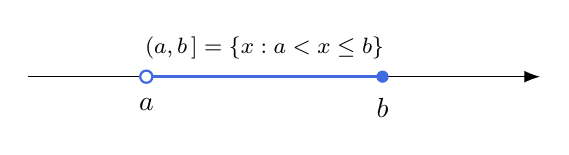
\begin{tikzpicture}[scale=1]
  \draw[-{Latex[length=2mm]}] (-0.5,0) -- (6,0);
  \foreach \x/\l in {1/a,4/b} \node[below] at (\x,-0.15) {$\l$};
  \draw[very thick,RoyalBlue] (1,0)--(4,0);
  \fill[white,draw=RoyalBlue,thick] (1,0) circle (2.2pt); % open at a
  \fill[RoyalBlue] (4,0) circle (2.2pt);                  % closed at b
  \node[above,font=\footnotesize] at (2.5,0.1) {$(a,b\,]=\{x: a<x\le b\}$};
\end{tikzpicture}
\end{center}

\[
\begin{array}{ll}
[a,b]=\{x:a\le x\le b\} & \text{closed (both ends in)}\\
(a,b)=\{x:a<x<b\} & \text{open (both ends out)}\\
{[a,b)}=\{x:a\le x<b\},\quad (a,b]=\{x:a<x\le b\} & \text{half-open}\\
{[a,\infty)}=\{x:x\ge a\},\quad (-\infty,b)=\{x:x<b\} & \text{unbounded}\\
(-\infty,\infty)=\R & \text{the whole line}
\end{array}
\]
$\infty$ is \emph{not} a number, only a direction --- so it is \emph{always} paired
with a parenthesis, never a bracket.

\begin{example}
Solve $|x-3|<2$ and write the solution as an interval.
\[
|x-3|<2 \iff -2<x-3<2 \iff 1<x<5 \iff x\in(1,5).
\]
\end{example}

\subsection{Absolute value and distance on the line}
The \textbf{absolute value} $|x|$ is the distance from $x$ to $0$:
\[
|x|=\begin{cases} x, & x\ge 0\\ -x, & x<0.\end{cases}
\]
The distance between two real numbers is $|a-b|$. Useful facts:
$|xy|=|x|\,|y|$, and the \textbf{triangle inequality} $|x+y|\le|x|+|y|$.

\lookahead{$|a-b|$ is distance in one dimension. In Unit~2 we generalize it to a
\emph{norm} $\|x-y\|$, which measures distance between vectors --- and the
triangle inequality survives unchanged.}

%==============================================================================
\section{Functions}
%==============================================================================
A \textbf{function} $f:A\to B$ assigns to each input $x\in A$ exactly one output
$f(x)\in B$. Here $A$ is the \textbf{domain}, $B$ the \textbf{codomain}, and
\[
\operatorname{range}(f)=\{f(x): x\in A\}\subseteq B
\]
is the set of values actually hit (the \textbf{image}).

\begin{example}
For $f:\R\to\R,\ f(x)=x^2$: the domain is $\R$, the codomain is $\R$, but the
range is $[0,\infty)$ because squares are never negative.
\end{example}

\textbf{Composition} feeds one function into another:
$(g\circ f)(x)=g\bigl(f(x)\bigr)$ --- do $f$ first, then $g$. An \textbf{inverse}
$f^{-1}$ undoes $f$: $f^{-1}(f(x))=x$. A function has an inverse exactly when it
is one-to-one (distinct inputs give distinct outputs).

\begin{example}
If $f(x)=2x+1$ then $f^{-1}(x)=\dfrac{x-1}{2}$, since solving $y=2x+1$ for $x$
gives $x=\frac{y-1}{2}$. Check: $f^{-1}(f(3))=f^{-1}(7)=3$. \checkmark
\end{example}

\lookahead{A \emph{linear transformation} (Unit~8) is a special kind of function
between vector spaces, and matrix multiplication is exactly \emph{composition} of
such functions. The matrix inverse (Unit~4) is a function inverse. Exponential
and logarithm (\S5) are inverses of each other.}

%==============================================================================
\section{Summation ($\Sigma$) and Product ($\Pi$) Notation}
%==============================================================================

\subsection{Sigma notation}
$\Sigma$ (capital sigma) is shorthand for a sum. The \textbf{index} $i$ runs from
the lower bound to the upper bound, and we add up the terms:
\[
\sum_{i=1}^{n} a_i \;=\; a_1+a_2+\cdots+a_n .
\]
The index name is a dummy: $\sum_{i=1}^{n}a_i=\sum_{k=1}^{n}a_k$.

\begin{example}
$\ds\sum_{i=1}^{4} i^2 = 1^2+2^2+3^2+4^2 = 30.$ \qquad
$\ds\sum_{k=0}^{3} 2^k = 1+2+4+8 = 15.$
\end{example}

\keybox{Algebra of sums (use these constantly)}{%
$\ds\sum_{i=1}^{n}(a_i+b_i)=\sum_{i=1}^{n}a_i+\sum_{i=1}^{n}b_i$ \quad(split a sum),\qquad
$\ds\sum_{i=1}^{n} c\,a_i = c\sum_{i=1}^{n}a_i$ \quad(pull out constants),\\[4pt]
$\ds\sum_{i=1}^{n} c = c\,n$ \quad(a constant term added $n$ times),\qquad
\emph{Index shift:} $\ds\sum_{i=1}^{n} a_i = \sum_{j=0}^{n-1} a_{j+1}$.}

The first two properties together are exactly \emph{linearity}, the single most
important structural fact in the whole course.

\begin{example}[Telescoping]
A sum where neighbors cancel:
\[
\sum_{i=1}^{n}\bigl(a_{i+1}-a_i\bigr)=a_{n+1}-a_1 .
\]
For instance $\sum_{i=1}^{n}\frac{1}{i(i+1)}=\sum_{i=1}^{n}\!\left(\frac1i-\frac1{i+1}\right)=1-\frac{1}{n+1}.$
\end{example}

\lookahead{The dot product $\langle x,y\rangle=\sum_i x_i y_i$ (Unit~2), the
matrix product, and every ``cost of an algorithm'' count (Unit~6) are written
with $\Sigma$. Linearity of the sum \emph{is} the reason these objects are called
``linear.''}

\subsection{Pi notation and factorials}
$\Pi$ (capital pi) is the same idea for \emph{products}:
\[
\prod_{i=1}^{n} a_i = a_1\cdot a_2\cdots a_n .
\]
The \textbf{factorial} is the product of the first $n$ positive integers:
\[
n! = \prod_{i=1}^{n} i = 1\cdot 2\cdot 3\cdots n,\qquad 0!=1 \ (\text{by convention}).
\]

\begin{example}
$\ds\prod_{i=1}^{4} i = 4! = 24.$ \qquad
$\ds\prod_{k=1}^{3}(2k) = 2\cdot4\cdot6 = 48.$
\end{example}

\lookahead{The determinant of a matrix is a signed sum of \emph{products} of
entries (Unit~4), and equals the \emph{product} of the eigenvalues
$\det A=\prod_i\lambda_i$ (Unit~11). Factorials reappear in the binomial theorem
(\S6) and Taylor's theorem (Unit~5).}

%==============================================================================
\section{Common Summation Formulas}
%==============================================================================
These closed forms turn a long sum into a single expression. Memorize the first
four; understand where the geometric series comes from.

\keybox{Closed forms}{%
$\ds\sum_{i=1}^{n} 1 = n$,\qquad
$\ds\sum_{i=1}^{n} i = \frac{n(n+1)}{2}$,\qquad
$\ds\sum_{i=1}^{n} i^2 = \frac{n(n+1)(2n+1)}{6}$,\qquad
$\ds\sum_{i=1}^{n} i^3 = \left(\frac{n(n+1)}{2}\right)^{\!2}$.\\[6pt]
\emph{Geometric:}\quad
$\ds\sum_{i=0}^{n} r^{i} = \frac{1-r^{\,n+1}}{1-r}\ (r\neq 1)$,\qquad
$\ds\sum_{i=0}^{\infty} r^{i} = \frac{1}{1-r}\ (|r|<1)$.\\[6pt]
\emph{Arithmetic:}\quad
$\ds\sum_{i=0}^{n-1}(a+id) = na + d\,\frac{n(n-1)}{2}$ \ (first term $a$, common difference $d$).}

\begin{example}[The Gauss pairing trick]
Why is $\sum_{i=1}^n i=\frac{n(n+1)}{2}$? Write the sum forwards and backwards and
add columns:
\[
\begin{array}{ccccccc}
S &=& 1 &+& 2 &+\cdots+& n\\
S &=& n &+& (n{-}1) &+\cdots+& 1\\ \hline
2S &=& (n{+}1) &+& (n{+}1) &+\cdots+& (n{+}1)
\end{array}
\]
There are $n$ copies of $(n+1)$, so $2S=n(n+1)$ and $S=\frac{n(n+1)}{2}$. (Legend
says Gauss found this as a schoolboy.)
\end{example}

\begin{example}[Using the formulas]
\[
\sum_{i=1}^{10} i = \frac{10\cdot 11}{2}=55,\qquad
\sum_{i=1}^{5} i^2=\frac{5\cdot 6\cdot 11}{6}=55,\qquad
\sum_{i=0}^{4} \Bigl(\tfrac12\Bigr)^{i}=\frac{1-(1/2)^5}{1-1/2}=\frac{31}{16}.
\]
\end{example}

\begin{example}[Infinite geometric series]
$\ds\sum_{i=0}^{\infty}\Bigl(\tfrac13\Bigr)^i=\frac{1}{1-\frac13}=\frac{3}{2}.$
The series converges only because $|r|=\frac13<1$; for $|r|\ge 1$ it diverges.
\end{example}

\lookahead{Summation formulas let us count operations in closed form: a double
loop over an $n\times n$ matrix costs $\sum_{i=1}^{n} n = n^2$ steps --- this is
how we get the ``$O(n^2)$'' and ``$O(n^3)$'' costs in Unit~6. The geometric series
also governs how fast iterative methods converge (Units~6, 11, 12).}

%==============================================================================
\section{Exponents and Logarithms}
%==============================================================================

\subsection{Exponent laws}
For a base $a>0$ and real exponents $m,n$:
\[
a^m a^n=a^{m+n},\quad \frac{a^m}{a^n}=a^{m-n},\quad (a^m)^n=a^{mn},\quad
(ab)^n=a^n b^n,\quad a^0=1,\quad a^{-n}=\frac{1}{a^n},\quad a^{1/n}=\sqrt[n]{a}.
\]

\begin{example}
$\ds 2^3\cdot 2^4 = 2^7 = 128$, \quad $\ds\frac{x^5}{x^2}=x^3$, \quad
$\ds (9)^{1/2}=3$, \quad $\ds 8^{-2/3}=\frac{1}{8^{2/3}}=\frac{1}{(\sqrt[3]{8})^2}=\frac14.$
\end{example}

\subsection{Logarithms: the inverse of exponentiation}
The logarithm answers ``\emph{to what power must I raise the base?}''
\[
\log_a x = y \iff a^{y}=x \qquad (a>0,\ a\neq 1,\ x>0).
\]
Two special bases: the \textbf{natural log} $\ln x=\log_e x$ (base $e\approx2.718$)
and, in computer science, $\log_2$.

\keybox{Logarithm laws (each mirrors an exponent law)}{%
$\ds\log_a(xy)=\log_a x+\log_a y$,\qquad
$\ds\log_a\!\frac{x}{y}=\log_a x-\log_a y$,\qquad
$\ds\log_a(x^r)=r\log_a x$,\\[4pt]
$\ds\log_a 1=0$,\qquad $\ds\log_a a=1$,\qquad
\emph{Change of base:}\ $\ds\log_a x=\frac{\ln x}{\ln a}$,\qquad
\emph{Inverses:}\ $a^{\log_a x}=x$ and $\log_a(a^x)=x$.}

\begin{example}
$\log_2 8 = 3$ since $2^3=8$. \quad $\ln(e^5)=5$. \quad
$\log_{10}(1000)=3$. \quad Using the laws,
$\log_2(3\cdot 8)=\log_2 3+\log_2 8=\log_2 3+3.$
\end{example}

\begin{example}[Solving with logs]
Solve $5\cdot 2^{x}=160$. Divide: $2^x=32$, so $x=\log_2 32 = 5$. \\
Solve $e^{3x}=10$. Take $\ln$: $3x=\ln 10$, so $x=\tfrac13\ln 10\approx 0.767$.
\end{example}

\subsection{What you should recall from MATH 141}
You will re-derive these in Unit~5, but keep them handy:
\[
\frac{d}{dx}\,e^{x}=e^{x},\qquad \frac{d}{dx}\,\ln x=\frac{1}{x}\ (x>0),\qquad
\frac{d}{dx}\,a^{x}=a^{x}\ln a.
\]
The number $e$ is special precisely because $e^x$ is its own derivative.

\lookahead{Logs turn products into sums --- which is why they tame the products of
many small probabilities in machine learning (the ``log-likelihood'' and
``cross-entropy loss'' of Unit~12). Exponentials define the matrix exponential
$e^{A}$ (Units~4, 11). And $\log_2$ measures how many times you can halve a
problem --- the source of ``$O(\log n)$'' running times (Unit~6).}

%==============================================================================
\section{Polynomials}
%==============================================================================
A \textbf{polynomial} of degree $n$ is a function
\[
p(x)=a_n x^n + a_{n-1}x^{n-1}+\cdots+a_1 x + a_0,\qquad a_n\neq 0,
\]
with the $a_i$ constants (\emph{coefficients}) and $a_n$ the \emph{leading}
coefficient. A \textbf{root} (or \emph{zero}) is a value $r$ with $p(r)=0$.

\keybox{Facts about roots}{%
\emph{Factor theorem:}\ $r$ is a root $\iff (x-r)$ divides $p(x)$.\\[2pt]
\emph{Quadratic formula:}\ the roots of $ax^2+bx+c=0$ are
$\ds x=\frac{-b\pm\sqrt{b^2-4ac}}{2a}$; the \emph{discriminant} $b^2-4ac$ is
$>0$ (two real roots), $=0$ (one repeated root), or $<0$ (two complex roots).\\[2pt]
\emph{Counting roots:}\ a degree-$n$ polynomial has \emph{exactly} $n$ roots in
$\C$, counted with multiplicity (Fundamental Theorem of Algebra).}

\begin{example}[Factoring]
$x^2-5x+6=(x-2)(x-3)$, so the roots are $x=2$ and $x=3$. Check with the factor
theorem: $p(2)=4-10+6=0$. \checkmark
\end{example}

\begin{example}[Quadratic formula \& complex roots]
Solve $x^2+x+1=0$. The discriminant is $1-4=-3<0$, so
$x=\dfrac{-1\pm\sqrt{-3}}{2}=-\dfrac12\pm\dfrac{\sqrt3}{2}\,i$ --- two complex
roots. (This is why we need $\C$; see Unit~3.)
\end{example}

\subsection{The binomial theorem}
Expanding $(x+y)^n$ uses \textbf{binomial coefficients}
$\displaystyle\binom{n}{k}=\frac{n!}{k!\,(n-k)!}$:
\[
(x+y)^n=\sum_{k=0}^{n}\binom{n}{k}x^{\,n-k}y^{\,k}.
\]

\begin{example}
$(x+y)^3=\binom30 x^3+\binom31 x^2 y+\binom32 x y^2+\binom33 y^3
= x^3+3x^2y+3xy^2+y^3.$
\end{example}

\lookahead{The \emph{characteristic polynomial} $\det(A-\lambda I)$ is a
degree-$n$ polynomial whose roots are the eigenvalues of a matrix (Unit~11). The
Fundamental Theorem of Algebra guarantees $n$ of them (possibly complex, possibly
repeated) --- which is exactly why eigenvalues can be complex even for a real
matrix.}

%==============================================================================
\section{Geometry: Distance and the Circle}
%==============================================================================

\subsection{The Pythagorean theorem}
In a right triangle with legs $a,b$ and hypotenuse $c$,
\[
a^2+b^2=c^2 .
\]

\begin{center}
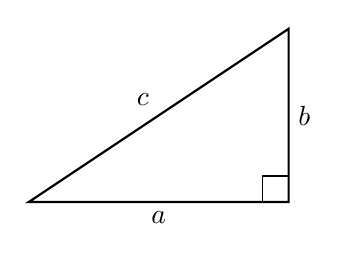
\begin{tikzpicture}[scale=1.1]
  \draw[thick] (0,0)--(3,0)--(3,2)--cycle;
  \draw (2.7,0)--(2.7,0.3)--(3,0.3); % right-angle mark
  \node[below] at (1.5,0) {$a$};
  \node[right] at (3,1) {$b$};
  \node[above left] at (1.5,1) {$c$};
\end{tikzpicture}
\end{center}

\begin{example}
Legs $3$ and $4$: $c=\sqrt{3^2+4^2}=\sqrt{25}=5$.
\end{example}

\subsection{The distance formula}
Applying Pythagoras to the horizontal and vertical gaps between two points gives
the distance in the plane, and the same idea extends to space:
\[
d\bigl((x_1,y_1),(x_2,y_2)\bigr)=\sqrt{(x_2-x_1)^2+(y_2-y_1)^2},
\]
\[
d\bigl((x_1,y_1,z_1),(x_2,y_2,z_2)\bigr)=\sqrt{(x_2-x_1)^2+(y_2-y_1)^2+(z_2-z_1)^2}.
\]

\begin{example}
The distance from $(1,2)$ to $(4,6)$ is $\sqrt{(4-1)^2+(6-2)^2}=\sqrt{9+16}=5$.
\end{example}

\lookahead{This is \emph{the} formula the course generalizes most. The
Euclidean norm $\|x\|_2=\sqrt{\sum_i x_i^2}$ (Unit~2) is just the distance formula
in $n$ dimensions, and least squares (Unit~10) minimizes exactly this distance
between a model and the data.}

\subsection{The equation of a circle}
A circle is the set of points at a fixed distance $r$ (the \emph{radius}) from a
center $(h,k)$. Setting ``distance to center $=r$'' and squaring:
\[
(x-h)^2+(y-k)^2=r^2 .
\]
Centered at the origin this is $x^2+y^2=r^2$. The 3-D analog is the \textbf{sphere}
$(x-h)^2+(y-k)^2+(z-l)^2=r^2$.

\begin{center}
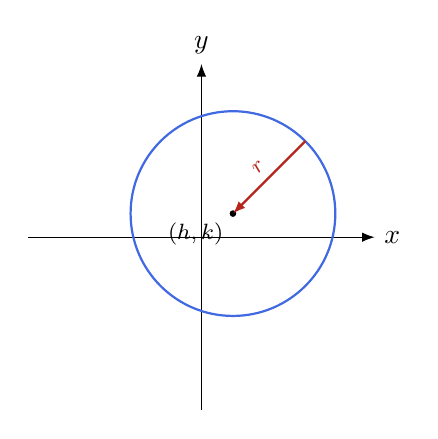
\begin{tikzpicture}[scale=1]
  \draw[-{Latex[length=1.6mm]}] (-2.2,0)--(2.2,0) node[right]{$x$};
  \draw[-{Latex[length=1.6mm]}] (0,-2.2)--(0,2.2) node[above]{$y$};
  \draw[thick,RoyalBlue] (0.4,0.3) circle (1.3);
  \fill (0.4,0.3) circle (1.2pt) node[below left,font=\footnotesize]{$(h,k)$};
  \draw[{Latex[length=1.6mm]}-,BrickRed,thick] (0.4,0.3)--(1.32,1.22)
      node[midway,above,font=\footnotesize,sloped]{$r$};
\end{tikzpicture}
\end{center}

\begin{example}
$(x-1)^2+(y+2)^2=9$ is the circle with center $(1,-2)$ and radius $3$.
Conversely, complete the square on $x^2+y^2-6x+4y+9=0$:
\[
(x^2-6x+9)+(y^2+4y+4)=-9+9+4 \;\Rightarrow\; (x-3)^2+(y+2)^2=4,
\]
a circle of center $(3,-2)$, radius $2$.
\end{example}

\lookahead{``All points at distance $\le r$'' is a disk --- and in $n$ dimensions,
the set $\{x:\|x\|\le r\}$ is the \emph{unit ball} of a norm (Unit~2). Its shape
(round for $\ell_2$, diamond for $\ell_1$, square for $\ell_\infty$) explains why
different norms behave so differently in regularization and optimization (Unit~12).}

\subsection{A little trigonometry and the unit circle}
On the \textbf{unit circle} $x^2+y^2=1$, the point at angle $\theta$ (measured
counterclockwise from the positive $x$-axis) is $(\cos\theta,\sin\theta)$.

\begin{center}
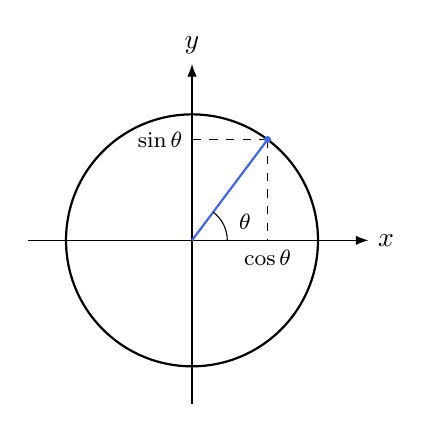
\begin{tikzpicture}[scale=1.6]
  \draw[-{Latex[length=1.6mm]}] (-1.3,0)--(1.4,0) node[right]{$x$};
  \draw[-{Latex[length=1.6mm]}] (0,-1.3)--(0,1.4) node[above]{$y$};
  \draw[thick] (0,0) circle (1);
  \draw[RoyalBlue,thick] (0,0)--(0.6,0.8);
  \draw[dashed] (0.6,0.8)--(0.6,0) node[below,font=\footnotesize]{$\cos\theta$};
  \draw[dashed] (0.6,0.8)--(0,0.8) node[left,font=\footnotesize]{$\sin\theta$};
  \fill[RoyalBlue] (0.6,0.8) circle (0.8pt);
  \draw (0.28,0) arc (0:53:0.28); \node[font=\footnotesize] at (0.42,0.15) {$\theta$};
\end{tikzpicture}
\end{center}

Because the point lies on the circle, we get the \textbf{Pythagorean identity}
\[
\cos^2\theta+\sin^2\theta=1,
\]
and $\tan\theta=\dfrac{\sin\theta}{\cos\theta}$. Angles are measured in
\textbf{radians}, where $180^\circ=\pi$; a few values worth knowing:
\[
\cos 0=1,\ \sin 0=0;\quad \cos\tfrac{\pi}{2}=0,\ \sin\tfrac{\pi}{2}=1;\quad
\cos\tfrac{\pi}{4}=\sin\tfrac{\pi}{4}=\tfrac{\sqrt2}{2}.
\]

\lookahead{The angle between two vectors (Unit~2) is measured with $\cos\theta$;
cosine \emph{similarity} in machine learning is exactly this $\cos\theta$.
Rotations in the plane, complex multiplication (Unit~3), and quaternions all run
on $\sin$ and $\cos$.}

\subsection{Lines in the plane}
A non-vertical line has \textbf{slope} $m=\dfrac{\Delta y}{\Delta x}=\dfrac{y_2-y_1}{x_2-x_1}$
and can be written
\[
y=mx+b \quad(\text{slope--intercept}),\qquad
y-y_1=m(x-x_1)\quad(\text{point--slope}).
\]

\begin{example}
The line through $(1,2)$ and $(3,8)$ has slope $m=\frac{8-2}{3-1}=3$, so
$y-2=3(x-1)$, i.e.\ $y=3x-1$.
\end{example}

\lookahead{A line is the graph of a \emph{linear} equation in two variables. A
\emph{system} of such equations is the starting point of the entire course
(Unit~7), and fitting the ``best'' line through scattered data is linear
regression (Unit~10).}

%==============================================================================
\section{Greek Alphabet and Symbol Glossary}
%==============================================================================
Linear algebra borrows heavily from Greek. You do not need to memorize this ---
just know where to look.

\begin{center}
\renewcommand{\arraystretch}{1.2}
\begin{tabular}{@{}llll@{}}
\toprule
\textbf{Symbol} & \textbf{Name} & \textbf{Symbol} & \textbf{Name}\\
\midrule
$\alpha$ & alpha & $\lambda$ & lambda (\emph{eigenvalues})\\
$\beta$ & beta & $\mu$ & mu (mean)\\
$\gamma$ & gamma & $\sigma,\ \Sigma$ & sigma (\emph{singular values} / \emph{sum})\\
$\delta,\ \Delta$ & delta (small change) & $\pi,\ \Pi$ & pi (\emph{product})\\
$\varepsilon$ & epsilon (tiny quantity) & $\phi,\varphi$ & phi\\
$\theta$ & theta (angle) & $\psi$ & psi\\
$\kappa$ & kappa (\emph{condition number}) & $\omega,\ \Omega$ & omega\\
\bottomrule
\end{tabular}
\end{center}

\begin{center}
\renewcommand{\arraystretch}{1.2}
\begin{tabular}{@{}ll@{\hspace{2em}}ll@{}}
\toprule
\textbf{Symbol} & \textbf{Meaning} & \textbf{Symbol} & \textbf{Meaning}\\
\midrule
$\in,\ \notin$ & is / is not an element of & $\forall$ & for all\\
$\subseteq,\ \subsetneq$ & subset / proper subset & $\exists$ & there exists\\
$\cup,\ \cap$ & union / intersection & $\Rightarrow$ & implies\\
$\varnothing$ & empty set & $\iff$ & if and only if\\
$\R,\ \C,\ \Z$ & reals, complex, integers & $\approx$ & approximately equals\\
$|x|,\ \|x\|$ & absolute value / norm & $\therefore$ & therefore\\
\bottomrule
\end{tabular}
\end{center}

%==============================================================================
\section{Self-Check (answers below)}
%==============================================================================
Work these with a pencil; if any feel shaky, reread the matching section.
\begin{enumerate}[leftmargin=1.6em,itemsep=3pt]
  \item Write $\{x\in\Z: -2\le x<3\}$ in roster form.
  \item With $A=\{1,2,3,4\},\ B=\{2,4,6\}$, find $A\cup B$, $A\cap B$, $A\setminus B$.
  \item Solve $|2x-1|\le 5$ and write the answer as an interval.
  \item Evaluate $\ds\sum_{i=1}^{6} i$ and $\ds\sum_{i=1}^{4} i^2$.
  \item Evaluate $\ds\sum_{k=0}^{\infty}\Bigl(\tfrac14\Bigr)^k$.
  \item Simplify $\log_2 40-\log_2 5$.
  \item Solve $3^{x}=81$ and $e^{2x}=7$ (leave the second exact).
  \item Find the roots of $x^2-4x+13=0$.
  \item Find the distance from $(-1,3)$ to $(2,-1)$.
  \item Give the center and radius of $x^2+y^2+4x-6y+9=0$.
\end{enumerate}

\subsection*{Answers}
\small
\begin{enumerate}[leftmargin=1.6em,itemsep=1pt]
  \item $\{-2,-1,0,1,2\}$.
  \item $A\cup B=\{1,2,3,4,6\}$, \ $A\cap B=\{2,4\}$, \ $A\setminus B=\{1,3\}$.
  \item $-5\le 2x-1\le 5\Rightarrow -2\le x\le 3$, i.e.\ $[-2,3]$.
  \item $\sum_{i=1}^6 i=\frac{6\cdot7}{2}=21$; \ $\sum_{i=1}^4 i^2=\frac{4\cdot5\cdot9}{6}=30$.
  \item $\frac{1}{1-1/4}=\frac{4}{3}$.
  \item $\log_2\frac{40}{5}=\log_2 8=3$.
  \item $x=4$ (since $3^4=81$); \ $x=\tfrac12\ln 7$.
  \item Discriminant $16-52=-36$, so $x=\frac{4\pm 6i}{2}=2\pm 3i$.
  \item $\sqrt{(2-(-1))^2+(-1-3)^2}=\sqrt{9+16}=5$.
  \item Complete the square: $(x+2)^2+(y-3)^2=4$; center $(-2,3)$, radius $2$.
\end{enumerate}
\normalsize

\vspace{0.6em}
\noindent\rule{\linewidth}{0.4pt}\\[2pt]
{\footnotesize\sffamily That is the whole toolkit. If the self-check went well,
you are ready for Unit~1. Keep this sheet nearby --- every symbol here reappears in
the first three weeks.}

\end{document}
